\documentclass[tikz,border=4pt]{standalone}
\usepackage{pgfplots}
\usepgfplotslibrary{groupplots}
\pgfplotsset{compat=1.18}
\definecolor{proposedblue}{RGB}{46,94,170}
\definecolor{staticgray}{RGB}{128,136,148}
\definecolor{oraclegreen}{RGB}{69,145,98}
\definecolor{blackboxorange}{RGB}{218,132,55}
\definecolor{nomarginred}{RGB}{186,78,68}
\definecolor{vacationgold}{RGB}{204,151,55}
\definecolor{monepurple}{RGB}{126,93,159}
\definecolor{tealgreen}{RGB}{35,143,135}
\definecolor{deepviolet}{RGB}{98,80,154}
\begin{document}

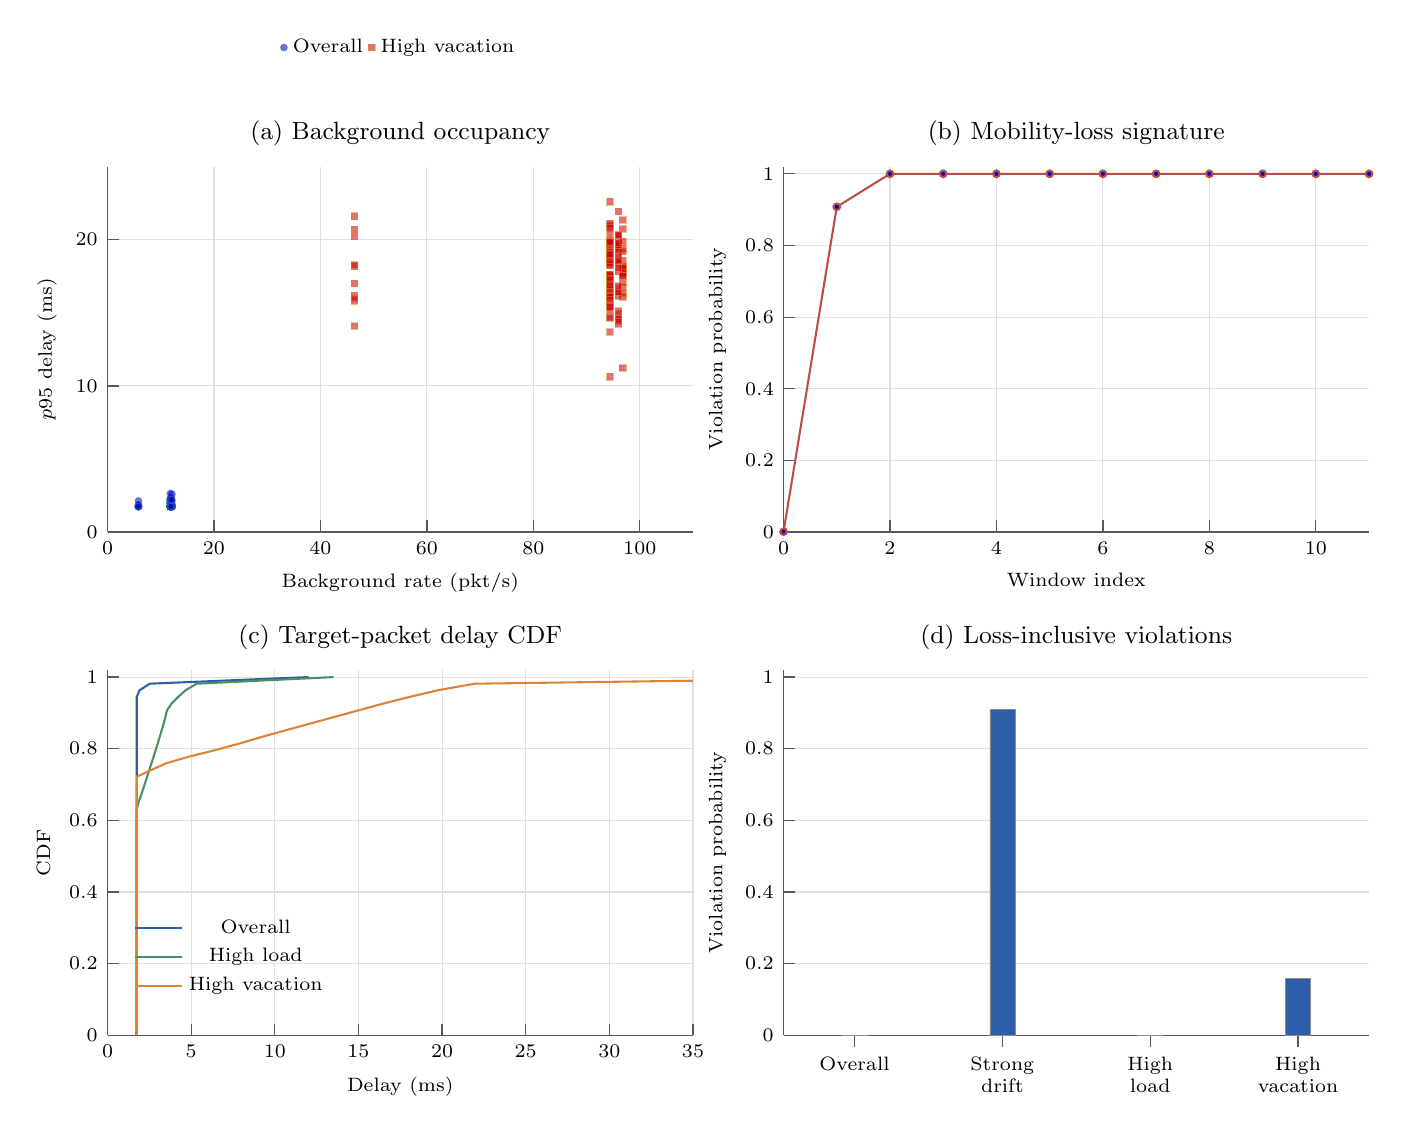
\begin{tikzpicture}
\begin{groupplot}[
    group style={group size=2 by 2, horizontal sep=1.15cm, vertical sep=1.75cm},
    width=3.55in,
    height=2.45in,
    ymajorgrids=true,
    xmajorgrids=true,
    grid style={black!12},
    axis x line*=bottom,
    axis y line*=left,
    axis line style={black!65, line width=0.45pt},
    tick style={black!65, line width=0.45pt},
    label style={font=\scriptsize},
    tick label style={font=\scriptsize},
    title style={font=\small, yshift=-0.5ex},
]
\nextgroupplot[
    title={(a) Background occupancy},
    xlabel={Background rate (pkt/s)},
    ylabel={$p95$ delay (ms)},
    xmin=0, xmax=110,
    ymin=0, ymax=25,
    legend style={at={(0.5,1.27)}, anchor=south, legend columns=2, draw=none, fill=none, font=\scriptsize},
]
\addplot+[only marks, mark=*, mark size=1.2pt, opacity=0.55, proposedblue] coordinates {
(11.8000,1.7461)
(12.1000,2.6055)
(11.8000,1.7461)
(11.8000,1.7461)
(12.0000,2.1828)
(11.8000,1.7462)
(12.1000,1.7462)
(11.8000,1.7462)
(12.0000,2.3836)
(11.8000,1.7462)
(12.0000,1.7462)
(5.8000,1.7462)
(11.8000,1.7809)
(12.1000,1.7461)
(11.8000,1.7462)
(11.8000,1.7461)
(12.0000,1.7462)
(11.8000,1.7462)
(12.1000,1.7462)
(11.8000,2.0358)
(12.0000,1.9196)
(11.8000,1.7462)
(12.0000,1.7462)
(5.8000,1.7462)
(11.8000,2.0290)
(12.1000,1.7461)
(11.8000,1.7554)
(11.8000,1.7461)
(12.0000,1.7462)
(11.8000,1.7462)
(12.1000,1.7462)
(11.8000,2.0500)
(12.0000,1.7462)
(11.8000,1.7462)
(12.0000,1.7462)
(5.8000,1.7462)
(11.8000,2.0897)
(12.1000,1.7461)
(11.8000,1.7461)
(11.8000,1.7461)
(12.0000,1.7462)
(11.8000,2.2280)
(12.1000,1.7462)
(11.8000,1.7462)
(12.0000,1.8070)
(11.8000,1.9681)
(12.0000,1.7462)
(5.8000,1.7462)
(11.8000,2.2219)
(12.1000,1.7461)
(11.8000,1.7461)
(11.8000,1.7462)
(12.0000,1.7462)
(11.8000,1.7462)
(12.1000,1.8024)
(11.8000,1.7462)
(12.0000,2.1292)
(11.8000,1.7462)
(12.0000,1.7462)
(5.8000,1.8214)
(11.8000,1.7731)
(12.1000,1.8209)
(11.8000,1.7461)
(11.8000,1.8612)
(12.0000,1.7462)
(11.8000,1.7462)
(12.1000,1.7462)
(11.8000,1.9461)
(12.0000,1.7462)
(11.8000,1.7462)
(12.0000,1.7462)
(5.8000,1.7462)
(11.8000,1.7461)
(12.1000,1.9009)
(11.8000,2.1923)
(11.8000,1.7462)
(12.0000,1.7462)
(11.8000,1.7462)
(12.1000,1.7462)
(11.8000,2.1873)
(12.0000,1.7462)
(11.8000,1.7462)
(12.0000,1.7462)
(5.8000,1.8725)
(11.8000,1.7461)
(12.1000,1.7461)
(11.8000,1.7461)
(11.8000,1.7461)
(12.0000,1.7462)
(11.8000,1.7571)
(12.1000,1.7462)
(11.8000,1.7462)
(12.0000,1.7462)
(11.8000,1.7462)
(12.0000,2.2321)
(5.8000,1.7683)
(11.8000,1.7461)
(12.1000,1.8291)
(11.8000,1.7461)
(11.8000,1.7462)
(12.0000,1.7462)
(11.8000,1.7462)
(12.1000,1.7462)
(11.8000,2.0236)
(12.0000,1.7462)
(11.8000,1.7462)
(12.0000,1.7906)
(5.8000,2.1325)
(11.8000,2.3212)
(12.1000,2.1534)
(11.8000,1.7546)
(11.8000,2.6426)
(12.0000,1.7462)
(11.8000,1.7462)
(12.1000,1.7462)
(11.8000,1.7462)
(12.0000,2.2266)
(11.8000,1.7462)
(12.0000,1.7515)
(5.8000,1.7462)
};
\addlegendentry{Overall}
\addplot+[only marks, mark=square*, mark size=1.2pt, opacity=0.55, blackboxorange] coordinates {
(94.4000,15.4517)
(96.8000,11.2340)
(94.4000,18.5005)
(94.4000,15.8060)
(96.0000,14.9012)
(94.4000,20.8481)
(96.8000,18.1407)
(94.4000,18.4896)
(96.0000,18.3128)
(94.4000,19.2230)
(96.0000,20.2124)
(46.4000,18.1829)
(94.4000,17.4615)
(96.8000,16.7306)
(94.4000,18.6412)
(94.4000,16.6038)
(96.0000,19.3577)
(94.4000,19.4210)
(96.8000,19.3855)
(94.4000,19.8970)
(96.0000,14.6990)
(94.4000,21.1147)
(96.0000,19.3453)
(46.4000,16.1805)
(94.4000,18.7046)
(96.8000,18.0538)
(94.4000,19.7682)
(94.4000,16.0945)
(96.0000,16.6786)
(94.4000,16.2849)
(96.8000,16.0813)
(94.4000,18.7550)
(96.0000,16.4543)
(94.4000,18.4458)
(96.0000,21.9310)
(46.4000,15.8007)
(94.4000,16.1984)
(96.8000,16.3111)
(94.4000,17.5411)
(94.4000,15.4669)
(96.0000,17.8432)
(94.4000,16.3055)
(96.8000,18.5587)
(94.4000,14.7219)
(96.0000,18.7366)
(94.4000,17.2060)
(96.0000,20.3333)
(46.4000,15.9928)
(94.4000,17.3587)
(96.8000,21.3579)
(94.4000,18.2637)
(94.4000,16.8055)
(96.0000,19.6353)
(94.4000,19.7135)
(96.8000,20.7386)
(94.4000,21.0266)
(96.0000,15.0998)
(94.4000,18.2370)
(96.0000,18.4653)
(46.4000,20.6989)
(94.4000,15.1508)
(96.8000,18.1644)
(94.4000,10.6329)
(94.4000,19.7073)
(96.0000,14.5811)
(94.4000,19.6067)
(96.8000,17.7667)
(94.4000,17.0185)
(96.0000,19.2920)
(94.4000,19.1807)
(96.0000,19.6377)
(46.4000,14.0936)
(94.4000,18.8487)
(96.8000,19.1910)
(94.4000,19.7713)
(94.4000,20.3582)
(96.0000,19.7582)
(94.4000,17.4283)
(96.8000,17.7656)
(94.4000,17.6057)
(96.0000,18.4621)
(94.4000,18.7587)
(96.0000,18.9061)
(46.4000,21.6072)
(94.4000,14.6570)
(96.8000,17.0715)
(94.4000,22.5987)
(94.4000,18.3862)
(96.0000,16.1646)
(94.4000,16.1304)
(96.8000,18.0635)
(94.4000,20.7868)
(96.0000,14.2610)
(94.4000,17.4658)
(96.0000,16.4251)
(46.4000,18.2697)
(94.4000,17.6000)
(96.8000,17.7387)
(94.4000,18.6319)
(94.4000,16.5942)
(96.0000,16.8325)
(94.4000,18.9411)
(96.8000,17.5458)
(94.4000,19.0246)
(96.0000,20.3251)
(94.4000,19.8875)
(96.0000,18.5688)
(46.4000,20.2375)
(94.4000,19.8372)
(96.8000,17.5143)
(94.4000,16.9056)
(94.4000,17.2944)
(96.0000,19.7632)
(94.4000,15.3858)
(96.8000,19.8789)
(94.4000,13.6935)
(96.0000,18.0580)
(94.4000,15.9147)
(96.0000,14.4094)
(46.4000,17.0008)
};
\addlegendentry{High vacation}

\nextgroupplot[
    title={(b) Mobility-loss signature},
    xlabel={Window index},
    ylabel={Violation probability},
    xmin=0, xmax=11,
    ymin=0, ymax=1.02,
]
\addplot+[nomarginred, mark=*, mark size=1.2pt, line width=0.75pt] coordinates {
(0,0.0012)
(1,0.9079)
(2,1.0000)
(3,1.0000)
(4,1.0000)
(5,1.0000)
(6,1.0000)
(7,1.0000)
(8,1.0000)
(9,1.0000)
(10,1.0000)
(11,1.0000)
};

\nextgroupplot[
    title={(c) Target-packet delay CDF},
    xlabel={Delay (ms)},
    ylabel={CDF},
    xmin=0, xmax=35,
    ymin=0, ymax=1.02,
    legend style={at={(0.03,0.08)}, anchor=south west, legend columns=1, draw=none, fill=none, font=\scriptsize},
]
\addplot+[proposedblue, line width=0.75pt, mark=none] coordinates {
(1.7186,0.0000)
(1.7461,0.0185)
(1.7461,0.0370)
(1.7461,0.0556)
(1.7461,0.0741)
(1.7461,0.0926)
(1.7461,0.1111)
(1.7461,0.1296)
(1.7461,0.1481)
(1.7461,0.1667)
(1.7461,0.1852)
(1.7461,0.2037)
(1.7461,0.2222)
(1.7461,0.2407)
(1.7462,0.2593)
(1.7462,0.2778)
(1.7461,0.2963)
(1.7461,0.3148)
(1.7461,0.3333)
(1.7461,0.3519)
(1.7461,0.3704)
(1.7462,0.3889)
(1.7462,0.4074)
(1.7462,0.4259)
(1.7462,0.4444)
(1.7462,0.4630)
(1.7462,0.4815)
(1.7462,0.5000)
(1.7462,0.5185)
(1.7462,0.5370)
(1.7462,0.5556)
(1.7462,0.5741)
(1.7462,0.5926)
(1.7462,0.6111)
(1.7462,0.6296)
(1.7462,0.6481)
(1.7462,0.6667)
(1.7462,0.6852)
(1.7462,0.7037)
(1.7462,0.7222)
(1.7462,0.7407)
(1.7462,0.7593)
(1.7462,0.7778)
(1.7462,0.7963)
(1.7462,0.8148)
(1.7462,0.8333)
(1.7462,0.8519)
(1.7462,0.8704)
(1.7462,0.8889)
(1.7462,0.9074)
(1.7462,0.9259)
(1.7462,0.9444)
(1.9111,0.9630)
(2.5273,0.9815)
(12.0254,1.0000)
};
\addlegendentry{Overall}
\addplot+[oraclegreen, line width=0.75pt, mark=none] coordinates {
(1.7182,0.0000)
(1.7461,0.0185)
(1.7461,0.0370)
(1.7461,0.0556)
(1.7461,0.0741)
(1.7461,0.0926)
(1.7461,0.1111)
(1.7461,0.1296)
(1.7461,0.1481)
(1.7461,0.1667)
(1.7462,0.1852)
(1.7462,0.2037)
(1.7462,0.2222)
(1.7462,0.2407)
(1.7462,0.2593)
(1.7462,0.2778)
(1.7462,0.2963)
(1.7462,0.3148)
(1.7462,0.3333)
(1.7462,0.3519)
(1.7462,0.3704)
(1.7462,0.3889)
(1.7462,0.4074)
(1.7462,0.4259)
(1.7462,0.4444)
(1.7462,0.4630)
(1.7462,0.4815)
(1.7462,0.5000)
(1.7462,0.5185)
(1.7462,0.5370)
(1.7462,0.5556)
(1.7462,0.5741)
(1.7462,0.5926)
(1.7462,0.6111)
(1.7462,0.6296)
(1.8388,0.6481)
(1.9776,0.6667)
(2.1095,0.6852)
(2.2395,0.7037)
(2.3697,0.7222)
(2.4974,0.7407)
(2.6242,0.7593)
(2.7524,0.7778)
(2.8780,0.7963)
(2.9999,0.8148)
(3.1207,0.8333)
(3.2396,0.8519)
(3.3571,0.8704)
(3.4617,0.8889)
(3.5559,0.9074)
(3.8288,0.9259)
(4.2162,0.9444)
(4.6607,0.9630)
(5.3251,0.9815)
(13.5113,1.0000)
};
\addlegendentry{High load}
\addplot+[blackboxorange, line width=0.75pt, mark=none] coordinates {
(1.7220,0.0000)
(1.7461,0.0185)
(1.7461,0.0370)
(1.7461,0.0556)
(1.7461,0.0741)
(1.7461,0.0926)
(1.7461,0.1111)
(1.7461,0.1296)
(1.7461,0.1481)
(1.7461,0.1667)
(1.7461,0.1852)
(1.7461,0.2037)
(1.7461,0.2222)
(1.7461,0.2407)
(1.7462,0.2593)
(1.7462,0.2778)
(1.7462,0.2963)
(1.7462,0.3148)
(1.7462,0.3333)
(1.7462,0.3519)
(1.7462,0.3704)
(1.7462,0.3889)
(1.7462,0.4074)
(1.7462,0.4259)
(1.7462,0.4444)
(1.7462,0.4630)
(1.7462,0.4815)
(1.7462,0.5000)
(1.7462,0.5185)
(1.7462,0.5370)
(1.7462,0.5556)
(1.7462,0.5741)
(1.7462,0.5926)
(1.7462,0.6111)
(1.7462,0.6296)
(1.7462,0.6481)
(1.7462,0.6667)
(1.7462,0.6852)
(1.7462,0.7037)
(1.7669,0.7222)
(2.6065,0.7407)
(3.5070,0.7593)
(4.8519,0.7778)
(6.4478,0.7963)
(7.9095,0.8148)
(9.2404,0.8333)
(10.6776,0.8519)
(12.1318,0.8704)
(13.5769,0.8889)
(15.0246,0.9074)
(16.4687,0.9259)
(18.0364,0.9444)
(19.7253,0.9630)
(21.9473,0.9815)
(50.8246,1.0000)
};
\addlegendentry{High vacation}

\nextgroupplot[
    title={(d) Loss-inclusive violations},
    ybar,
    ymin=0,
    ymax=1.02,
    ylabel={Violation probability},
    symbolic x coords={overall,drift_strong,load_high,vacation_high},
    xtick=data,
    xticklabels={{Overall},{Strong\\drift},{High\\load},{High\\vacation}},
    x tick label style={font=\scriptsize, align=center, text depth=0.25ex},
    enlarge x limits=0.16,
    xmajorgrids=false,
]
\addplot+[
    ybar,
    bar width=9pt,
    fill=proposedblue,
    draw=black!45,
    line width=0.2pt
] coordinates {
(overall,0.0002)
(drift_strong,0.9091)
(load_high,0.0002)
(vacation_high,0.1582)
};
\end{groupplot}
\end{tikzpicture}
\end{document}
